\documentclass{article}
\usepackage[T1]{fontenc}
\usepackage{lmodern}
\usepackage{graphicx}
\usepackage{amsmath,amssymb}
\usepackage[a4paper,margin=2cm]{geometry}
\usepackage[absolute,overlay]{textpos}
\setlength{\TPHorizModule}{1mm}
\setlength{\TPVertModule}{1mm}
\usepackage[indonesian]{babel}
\usepackage{hyperref}
\setlength{\emergencystretch}{2em}
% unit: Halaman 62

\begin{document}

% === Halaman 62 (llm) ===

PLANETCALC Online calculators

\vspace{10mm}

Hide information inside picture

\vspace{187.11mm}

Message

We are discovered. Flee at once

\vspace{5mm}

Source image

\begin{tabular}{|l|l|}
\hline
File & Size \\ \hline
sushi-text.png & 2Kb \hline
\end{tabular}

\vspace{5mm}

CALCULATE

% deskripsi: Screenshot antarmuka kalkulator online untuk menyembunyikan informasi di dalam gambar (steganografi) yang menampilkan kotak pesan, area unggah file gambar, dan tombol hitung.
% bbox normalisasi: [0.0600, 0.2900, 0.7100, 0.9200]
\begin{textblock*}{136.50mm}(12.60mm,86.13mm)
\noindent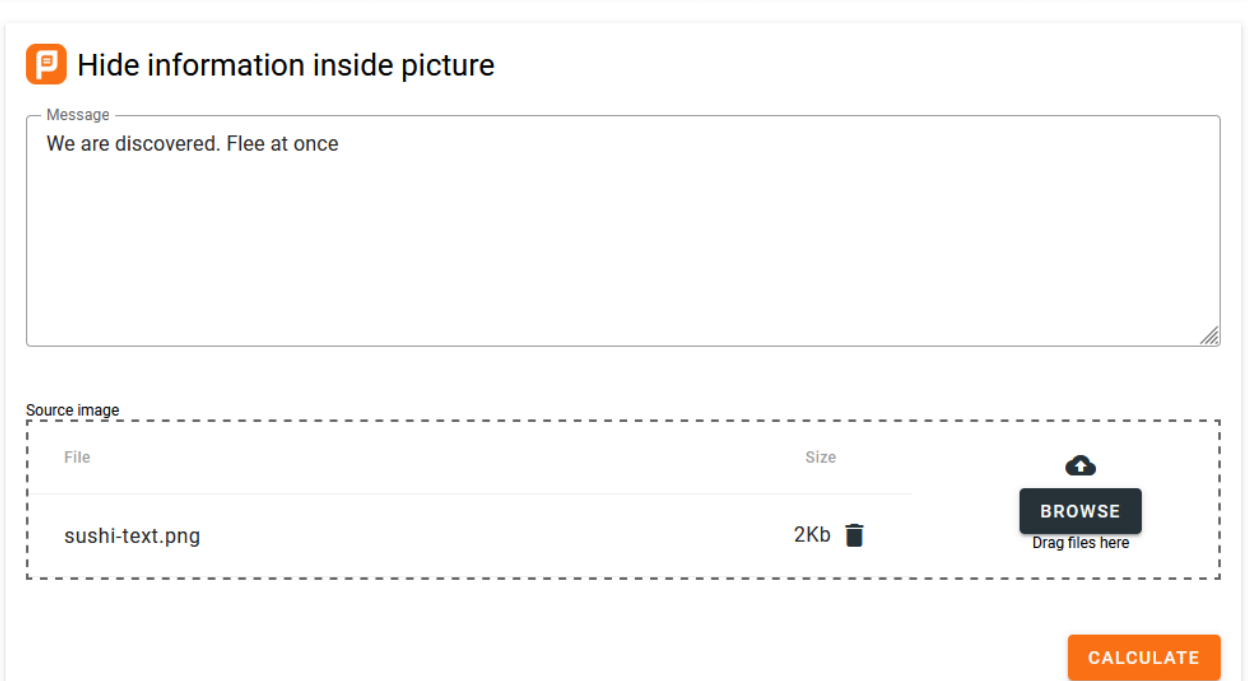
\includegraphics[width=136.50mm,height=187.11mm]{../../images/llm/page_062_img_01.png}%
\end{textblock*}

\end{document}
